\chapter{Machine Learning Models}
Machine learning is a scientific discipline focused on the development of algorithms focused on learning from examples. This idea has become central to the design of search engines, robots systems and forecasts applications which process large data sets. However, machines require an extended training period when developing algorithms to predict future behaviour such as financial time series forecasting where new data is available in a short period of time.  Online machine learning techniques tackle this problem and allow to update the model with new data or to compute a new model using less data allowing to give a response in a short period of time.

\vspace{0.5cm} 

\section{Introduction}
Machine Learning (ML) studies computer algorithms for learning
something such as to complete a task, to make accurate predictions or to behave intelligently. The learning is always based on samples and the objective is about to do better in the future based on the past experiences in an automatic way. ML is a subarea of artificial intelligence and broadly intersects with other fields such as statistics, mathematics, physics and computer science. 
There are many examples of machine learning problems: time series forecasting, image processing, face detection, spam filtering, weather prediction, search engines, among many others.

ML models are often more accurate than what can be created through direct programming. The reason is that ML models are data driven and are able to examine large amounts of data.

There are three types of ML classified depending on the nature of the learning input or output available to a learning system.
\begin{description}
\item[supervised learning]  the input data is a tuple which contains the example input and its desired outputs (also called labels). The list of tuples is called the training set. The concept of supervised learning comes from the supervisor, acting as a teacher in the learning process. The goal is to learn a general rule that maps inputs to outputs optimising a target function. There are two related problem types in supervised learning: classification and regression problems \cite{bishop2006}. Its two mainstream approaches are: support vector machines (SVMs) \cite{vapnik1998} and ensemble learning \cite{breiman1998}. Furthermore supervised learning can be categorised into offline or batch learning and online learning (see section \ref{sec:onoffline}). 
\item[unsupervised learning] also known as clustering \cite{ben2005}. In this type of learning no labels are given and the system has to find a structure on its own, discovering hidden patterns in data.
\item[reinforcement learning] is the problem faced by an agent that must learn 
through trial-and-error interactions with a dynamic environment. It is based on programming agents by reward and punishment without needing to specify how the task is to be achieved \cite{sutton1998}.
\end{description}



%%% Learning problem. Ac;a ma;ana, formulas y descripcion de tallada del problema de aprendizaje


\section{Statistical learning theory} \label{sec:mltheory}

All ML problems can be viewed as optimisation problems. The ML core task is to define a learning criterion, i.e the function to be optimised. 

In this thesis we will emphasised the supervised learning problem since it is the most common way of modelling financial problems.

Supervised learning consists in to find a learning function $f: X \rightarrow Y$ which models a set of examples called training set $S$ which have been drawn randomly and independently according to a unknown joint distribution function $p(x,y)$ on $X \times Y$:


$$
S= \{(x_1,y_1),\,(x_2,y_2),\dots\,,\,(x_n,y_n)\} \in \mathcal{S}, (x_i,y_i) \in X\times Y \quad \forall i = 1\dots n
$$

\noindent where $X \subseteq \mathbb{R}^m$ and $Y = \mathbb{R}$ in case of regression problems and $Y = \{1,-1\}$  if it is a classification problem. 

A learning algorithm $\mathcal{A}$ takes as input a data set $S \in \mathcal{S}$ and output a function $f_S$:

\begin{eqnarray*}
\mathcal{A}: \mathcal{S} &\rightarrow & \mathcal{H} \\
S &\rightarrow &\mathcal{A}(S) = f_S
\end{eqnarray*}

\noindent where $\mathcal{H}$ is called the hypothesis space, is the space of functions that the algorithm is allowed to search. The selection of $f_S$ is based on a loss function $V(f(x),y)$ which expected risk has to be minimised.

\[
E[V(f(x),y)] = \int V(f(x),y) dp(x,y)
\]

\noindent $V(f(x),y)$ denote the price paid for mistakes. Therefore, $V(f(x),y)=0$ if$f(x)=y$.

For regression, the most common loss function is square loss or L2 loss function:
\begin{equation}
\label{eq:l2loss}
V(f(x),y) = (f(x)-y)^2
\end{equation}
\noindent another option is the L1 loss
\begin{equation}
\label{eq:l1loss}
V(f(x),y) = |f(x)-y| \, .
\end{equation}
\noindent the choice of loss function here gives rise to several well-known learning algorithms such as regularised least squares and support vector machines. %verificar esto7776

Since the true distribution is unknown and only training samples are available, the objective is to estimate a function $\hat{f}$ through empirical risk (training error) minimisation (ERM): 

\begin{equation} 
\label{eq:erm}
R_{\text{emp}}[f] = \frac{1}{n} \sum_{i=1}^n V(f(x),y)
\end{equation}

\subsection{Learning algorithms}
In all learning algorithms that are trained from example data, there is a tradeoff \cite{dietterich2003} between three factors:
\begin{description}
\item[Complexity of the hypothesis class] for best generalisation, we should adjust the complexity of the learner model $\hat{f}$ to the complexity of the data $f$. In polynomial regression, the complexity parameter is the order of the fitted polynomial, and therefore we need to find a way to choose the best order that minimises the generalisation error, that is, tune the complexity of the model to best fit the complexity of the function inherent in the data.
\item[Generalisation accuracy on new examples] is the capability of the algorithm to generate the right output for an input instance outside the training set.
\item[The amount of training data]  generally generalisation accuracy increases as the amount of training data increases.
\end{description}

Very complex models will fit the training data better (low bias) but it could overfit it and generalise poorly (high variance), this is also called the bias-variance tradeoff.  Generalisation accuracy can sometimes be improved with more training data. The figure \ref{fig:tradeoff} illustrates how generalisation accuracy depends on the complexity of the model and the amount of training data.

\begin{figure}[!h]
  \centering
  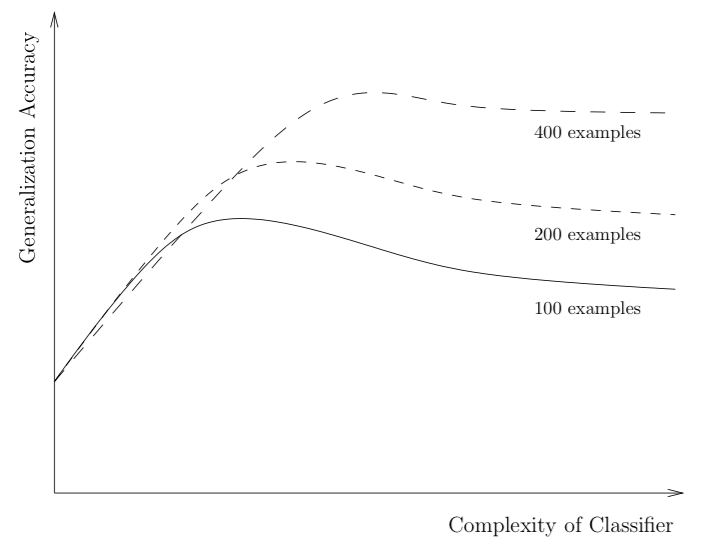
\includegraphics[width=0.8\textwidth]{img/3tradeoff}
  \caption{Triple tradeoff in empirical learning}
  \label{fig:tradeoff}
\end{figure}

\subsection{The bias-variance tradeoff}

Models learning error can be split into two main components: error due to bias and error due to variance. Bias measures how far off in general these models' predictions are from the correct value. Variance is taken as the variability of a model prediction for a given data point.

If we have a learning model $\hat{f}$, its expected generalisation error on an unseen or testing sample $x$ can be decomposed as follows:

\begin{align}
\mathrm{E}\Big[\big(y - \hat{f}(x)\big)^2\Big]
 & = \mathrm{Bias}\big[\hat{f}(x)\big]^2 + \mathrm{Var}\big[\hat{f}(x)\big] + \sigma^2
\end{align}
\noindent where:
\begin{align*}
 \mathrm{Bias}\big[\hat{f}(x)\big] &= \mathrm{E}\big[\hat{f}(x)\big] - f(x) \\
 \mathrm{Var}\big[\hat{f}(x)\big] &= \mathrm{E}\Big[ \big( \hat{f}(x) - \mathrm{E}[\hat{f}(x)] \big)^2 \Big] 
\end{align*}


Bias is introduced by the model selection. Therefore the model building process is repeated (through resampling) and substantially different averages of prediction values are obtained, bias will be high. The error due to variance is the amount by which the prediction, over one training set, differs from the expected predicted value, over all the training sets. Variance measures how inconsistent are the predictions from one another, over different training sets, not whether they are accurate or not.

This generalisation error is unknown, but it can be estimated using a training sample, a testing sample or by estimating the model complexity. Figure \ref{fig:traintesterror} shows prediction error for training and testing sample.  In general, in the training sample prediction error is decreasing with more complex models but it overfit the data and it is not a good model for the test data. Figure \ref{fig:bvtradeoff} shows how testing error can be decomposed into bias and variance components. The best model will be the one has a balance between bias and variance.

\begin{figure}[!h]
  \centering
  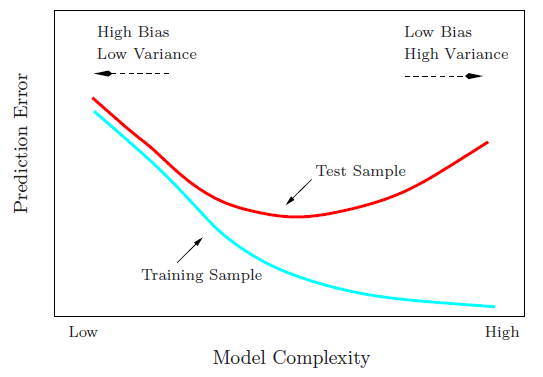
\includegraphics[width=0.8\textwidth]{img/model_complexity}
  \caption{Training and test error}
  \label{fig:traintesterror}
\end{figure}


The objective is to simultaneously reduce bias and variance as much as possible in order to obtain as accurate model as is feasible.  However, there is a tradeoff to be made when selecting models. Models that exhibit small variance and high bias underfit the truth target.  Models that exhibit high variance and low bias overfit the truth target.

This bias-variance tradeoff is the reason why in order to obtain the best model, data is usually broken in three subsets: training set, validation set and testing set. Training set is used to determine the model, validation set is used to estimate the generalisation error and finally testing set is used to estimate the accuracy of the model. Usually the partition is 50\% for training set, 25\% for validation and 25\% for testing purposes. This procedure can be extended to a Cross Validation (CV) procedure \cite{geisser1975}, usually used when the amount of data is limited. Various splitting strategies lead to various CV estimates. In K-fold cross-validation the training data is divided randomly into K distinct subsets, then the network is trained using K-1 subsets, and tested on the remaining subset. The process of training and testing is then repeated for each of the K possible choices of the subset omitted from the training. The average performance on the K omitted subsets is then our estimate of the generalisation performance.

\begin{figure}[!h]
  \centering
  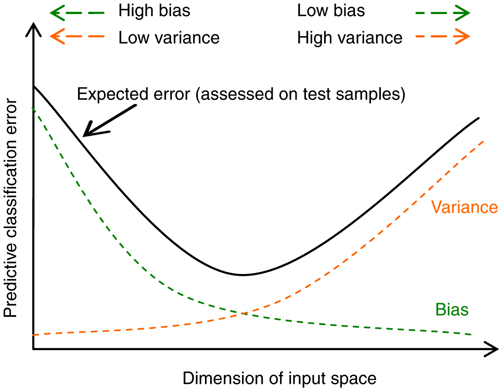
\includegraphics[width=0.8\textwidth]{img/biasvariancetradeoff}
  \caption{Bias variance tradeoff}
  \label{fig:bvtradeoff}
\end{figure}

Another way to control the complexity of the model is to include in the optimisation function not only the generalisation error but a penalisation of high complex models. 


\subsection{Regularization}
Since ERM is an ill-posed problem, Tikhonov introduced a regularisation which ensures well-posedness and generalisation of ERM, i.e prevents overfit, by constraining the hypothesis space $\mathcal{H}$ usually called regularised ERM or Tikhonov regularisation.

Tikhonov regularisation minimised over the hypothesis space $\mathcal{H}$ for a fixed positive parameter $\lambda$ the following:

\begin{equation} 
\label{eq:rerm}
R_{\text{emp}}[f] = \frac{1}{n} \sum_{i=1}^n V(f(x),y) + \lambda \mathcal{R}(f)
\end{equation}

\noindent where $\mathcal{R}(f)$ is the regulariser, a penalisation on $f$.

One example of regularisation in linear models is ridge regression, which is a regularised least squares method.
The least squares (LS) method is a well known way to solve a regression
problem. 
LS method consists of minimising the sum of squared errors:

%\begin{eqnarray*}
%\label{eq:problem2}
% J(\mathbf{\phi}) &=& \sum_{t=1}^N (f(\mathbf{x}_t)-y_t)^2 
% = \sum_{t=1}^N (\mathbf{\phi}^\intercal {\mathbf{x}}_t-y_t)^2 
% = \| \mathbf{X}\mathbf{\phi} - \mathbf{Y} \|_2^2 
%\end{eqnarray*}

% Aca seguir agregando slides.tex

\section{Batch and Online learning} \label{sec:onoffline}

Batch learning, also called statistical or offline learning, is a supervised machine learning framework. In batch learning, there is a data set available where the learner can build the internal model without any limits in accessing the data. There is time enough to carefully analyse the dataset, build large predictive models and combine them in a sophisticated way. 


In contrast to offline learning, online learning has access to a sample only once. The goal is the same, predicting targets as accurate as possible. For example, stock market prediction can be seen as online learning. The algorithm makes a prediction of the stock, little time after the real stock price is available, this information can be incorporated to the learner to further improve the prediction accuracy. In general, there is very much data available in an online learning setup, the data set grows continuously. Offline learning has equal or superior accuracy compared to online learning when the same amount of data is used.


\subsection{Online learning}

Classic statistical theory of sequential prediction enforces strong assumptions on the statistical properties of the input sequence (for example, stationary stochastic process). However, these assumptions can be unknown or change over time. In online learning there is no previous assumption about the data and the sequence is allowed to be deterministic, stochastic or even adaptive.  

Moreover, in case we receive data streams, ANN or SVM cannot introduce new information into the model without a re-training process, so we will have to use the same non-updated model until we decide to compute another one if it is possible.  Online learning algorithms allow one example at a time to be introduced into an existing model incrementally~\cite{vovk2005}. This is extremely important when the problem has large data streams and real-time forecasting must be done.  This is the most common scenario when we want to forecast a wide range of data such as stock prices and volatilities, electricity power, intrusion detection, web-mining, server load, etc.  Besides, many problems of high interest in machine learning can be treated as online ones and they can also use these types of algorithms.

The online learning framework was first introduced in the perceptron algorithm~\cite{rosenblatt58}. There are several other widely used online methods such as passive-aggressive~\cite{crammerETall2006}, stochastic gradient descent~\cite{zhang2004}, aggregating algorithm~\cite{vovk2001} and the second order perceptron~\cite{cesa-bianchi2005}.  In~\cite{cesa-bianchi2006} an in-depth analysis of online learning is provided.

The motivation for online learning is to obtain computational efficiency and tackle the shifting problem, i.e. that the distribution of the data is unknown or changes over time. Online learning algorithms can deal with this problem because they have a tracking ability which is a strategy based on retaining weak dependence on past examples by using two types of models: 

\textit{a)} \textbf{memory boundedness:} consists of limiting the number of support vectors in order to improve computational efficiency. One example of this is the budget perceptron~\cite{crammeretal2004} which reduces the number of examples used for prediction. Alternatively, in the forgetron algorithm~\cite{dekeletal2008} the damage caused by removing old examples is discussed, which can be avoided by removing samples with small influences. Other examples are the sliding window kernel (RLS)~\cite{vanvaerenberghetal2006}, which only considers a sliding window of the most recent data, and in \cite{arce+salinas2012} is shown a variant of aggregating algorithm for regression~\cite{vovk2001} considering only a sliding window of the most recent data, optimising also common matrix operations.

\textit{b)} \textbf{weight decay:} one example of this is the shifting perceptron algorithm which implements an exponential decaying scheme for the examples~\cite{cavallantietal2007}.
Performance of an online learning algorithm is measured by the cumulative loss it suffers along its run on a sequence of examples. In order to minimise this loss, the learner may update the hypothesis after each round so as to be more accurate in later rounds.

%%% Measure error
